\documentclass[tikz,border=6pt]{standalone}
\usepackage[T1]{fontenc}
\usepackage[utf8]{inputenc}
\usepackage{pgfplots}
\usepgfplotslibrary{groupplots}
\usetikzlibrary{calc}
\pgfplotsset{compat=1.18}
\begin{document}
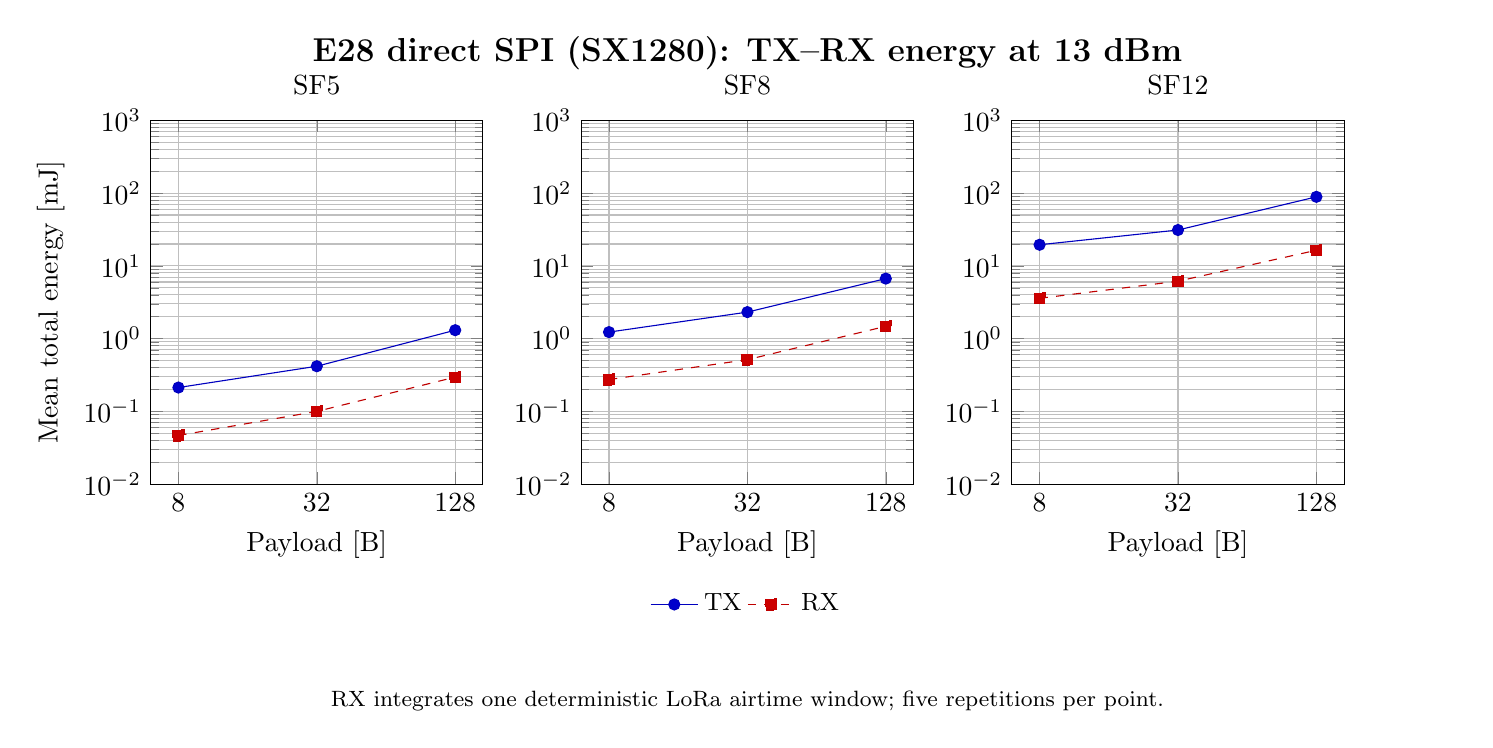
\begin{tikzpicture}
\begin{groupplot}[/pgf/number format/use comma, group style={group size=3 by 1, horizontal sep=1.25cm},
  width=5.8cm,height=6.2cm,xmode=log,log basis x=2,ymode=log,log basis y=10,ymin=0.01,ymax=1000,
  xtick={8,32,128},xticklabels={8,32,128},grid=both,xlabel={Payload [B]},
  legend style={draw=none,fill=none,font=\small,at={(0.5,-0.27)},anchor=north,legend columns=-1}]
% TX--RX energy
\nextgroupplot[title={SF5},ylabel={Mean total energy [mJ]}]
\addplot+[blue!75!black,solid,mark=*,error bars/.cd,y dir=both,y explicit] coordinates {(8,0.21244352) +- (0,0.00107057463) (32,0.416920492) +- (0,0.00175434231) (128,1.30580825) +- (0,0.00139394468)};
\addplot+[red!75!black,dashed,mark=square*,error bars/.cd,y dir=both,y explicit] coordinates {(8,0.0465523111) +- (0,0.000366978495) (32,0.0997945881) +- (0,0.0010975085) (128,0.295300695) +- (0,0.00134052199)};
\nextgroupplot[title={SF8}]
\addplot+[blue!75!black,solid,mark=*,error bars/.cd,y dir=both,y explicit] coordinates {(8,1.22908945) +- (0,0.00317393486) (32,2.31463865) +- (0,0.00788799703) (128,6.68808069) +- (0,0.0215877545)};
\addlegendentry{TX}
\addplot+[red!75!black,dashed,mark=square*,error bars/.cd,y dir=both,y explicit] coordinates {(8,0.273615791) +- (0,0.00246646567) (32,0.513640634) +- (0,0.00334195347) (128,1.47579347) +- (0,0.00726719607)};
\addlegendentry{RX}
\nextgroupplot[title={SF12}]
\addplot+[blue!75!black,solid,mark=*,error bars/.cd,y dir=both,y explicit] coordinates {(8,19.522688) +- (0,0.0579098323) (32,31.142606) +- (0,0.0983942111) (128,89.0247703) +- (0,0.274420996)};
\addplot+[red!75!black,dashed,mark=square*,error bars/.cd,y dir=both,y explicit] coordinates {(8,3.58193322) +- (0,0.00606049209) (32,6.15891566) +- (0,0.0124518885) (128,16.4082026) +- (0,0.0468163593)};
\end{groupplot}
\node[font=\bfseries\large] at ($(group c2r1.north)+(0,0.85cm)$) {E28 direct SPI (SX1280): TX--RX energy at 13 dBm};
\node[font=\footnotesize,align=center,text width=18cm] at ($(group c2r1.south)+(0,-2.75cm)$) {RX integrates one deterministic LoRa airtime window; five repetitions per point.};
\end{tikzpicture}
\end{document}
